\chapter{General introduction}\thumbforchapter
\newpage

\section{The central dogma of molecular biology}

All cells within our body share the same DNA, yet they display remarkable diversity and specialization. How, then, can a single set of genetic instructions (DNA) give rise to such diverse cell types? Consider the complexity of the human body, composed of an estimated 37 trillion cells (Bianconi et al., 2013). Each of these cells contains approximately 2 meters of DNA, collectively forming an astounding 74,000,000,000 kilometers of genetic material, equivalent to nearly 250 round trips to the sun! This genetic information is distributed across 23 distinct structures known as chromosomes and contains roughly 20,000 genes. What is the role of evolution in this process, and consequently, what are the differences in instructions between species? To better understand these fascinating phenomena, it is crucial to understand the central dogma of molecular biology (fig. \ref{fig:central_dogma}).

\begin{figure}[H]
    \center
    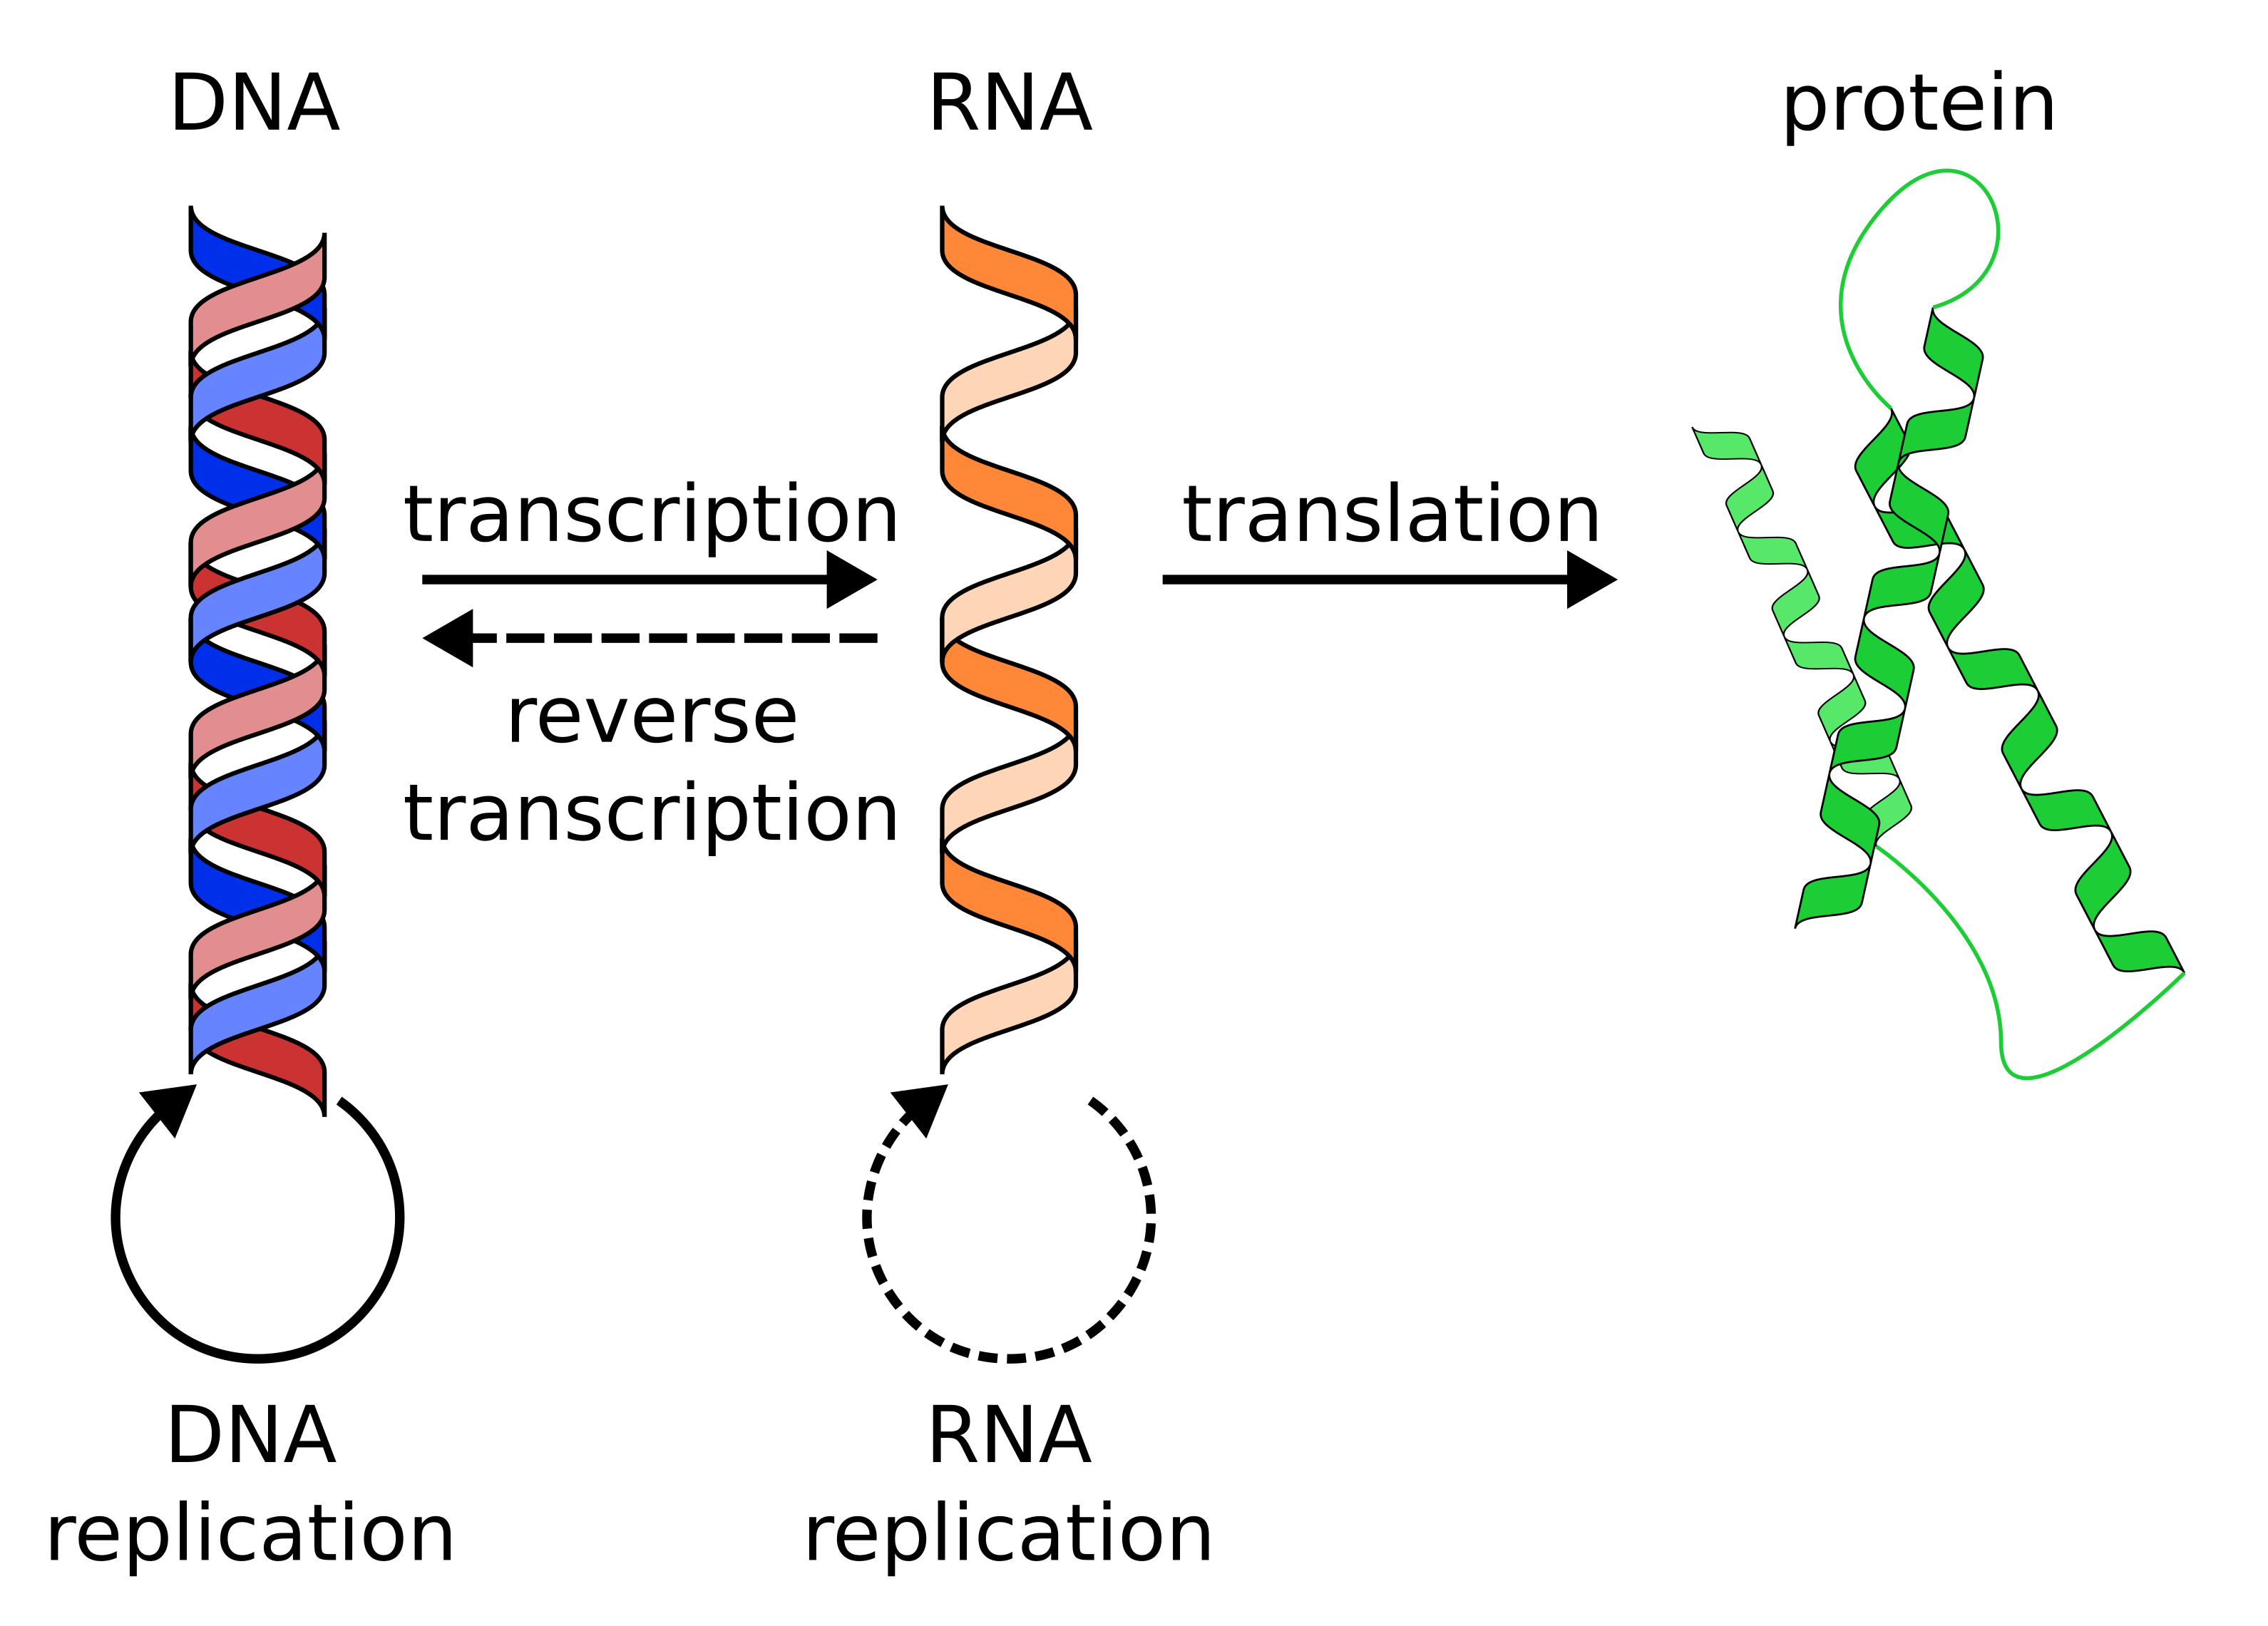
\includegraphics[width=0.7\linewidth]{ch.introduction/imgs/central_dogma.png}
    \caption{\textbf{The central dogma of molecular biology.} DNA transcribes to RNA, and RNA translates to protein. Solid arrows indicate the general flow of information in the system, and dotted arrows are special cases.}
    \label{fig:central_dogma}
\end{figure}

The central dogma of molecular biology describes the flow of genetic information within a biological system. Whereas in a computer information is stored in bits, which can be either zero (0) or one (1), genetic information is stored in nucleotides, which can be either adenine (A), cytosine (C), guanine (G), or thymine (T). DNA is composed of two large strands of these four nucleotides that together form a double helix. Both strands contain the same information, but where there is a nucleotide A on one strand, there is always a corresponding nucleotide T on its complementary strand, and similarly for C and G. RNA, on the other hand, is a similar molecule but is typically single-stranded. It is transcribed from DNA and shares a similar nucleotide composition but replaces thymine (T) with uracil (U). RNA serves as the bridge between DNA and proteins. Through the process of translation, the information encoded in RNA is decoded and used to assemble chains of amino acids, known as proteins. Proteins carry out various tasks in our bodies, such as enabling chemical reactions, transporting other molecules, providing structure, and acting as regulators of DNA transcription and RNA translation.

Far from all the human DNA is transcribed to RNA, and not even all RNA translates to protein. As a general rule of thumb, we distinguish DNA sequences that get transcribed into RNA as genes. The human genome contains approximately 20,000 protein-coding genes, and these genes cover only 1.5\% of the genome\cite{Piovesan2019}. Early molecular biologists mainly focused on protein-coding genes, thus the remaining 98.5\% of the DNA got known as ``junk DNA'', a controversial term in the field\cite{Graur2013}. Recent research has revealed that around 10\% of human DNA is functional\cite{Graur2013}, although some estimates suggest that 
as much as 80\% of DNA plays a role in at least one biochemical process\cite{encode2012}.

\section{Gene expression regulation}

Even though all cells of an organism contain identical DNA, they use completely different sets of genes. This is possible due to the tight regulation of gene expression, for which cells have a wide array of tools at their disposal. This thesis mainly focuses on transcription factors in gene regulation and chromatin context.

\subsection{Transcription Factors}

A typical gene consists of its coding regions (exons), noncoding regions (introns), and the start site (promoter). The promoter functions as a location where general transcription factors (GTFs) bind, which in turn recruit RNA polymerase II (RNAPII). RNAPII is the protein complex responsible for transcription and is responsible for reading out the DNA of a gene and converting it to RNA. Even though the presence of general transcription factors and a promoter is generally enough for transcription to occur\cite{Haberle2018}, its regulation occurs through the interplay of transcription factors and enhancers (figure \ref{fig:TF}). Enhancers are small regions on the DNA, typically a few hundred base pairs in length. TFs bind in these enhancers, based on specific DNA sequences (motifs). Different TFs have different functions, and some help with the recruitment of RNAPII and GTFs, whilst others help with making the promoter or other DNA sequences more accessible. Transcription factors thus act like switches, determining whether transcription should be turned up or down in response to various signals and conditions.

\begin{figure}[h]
    \center
    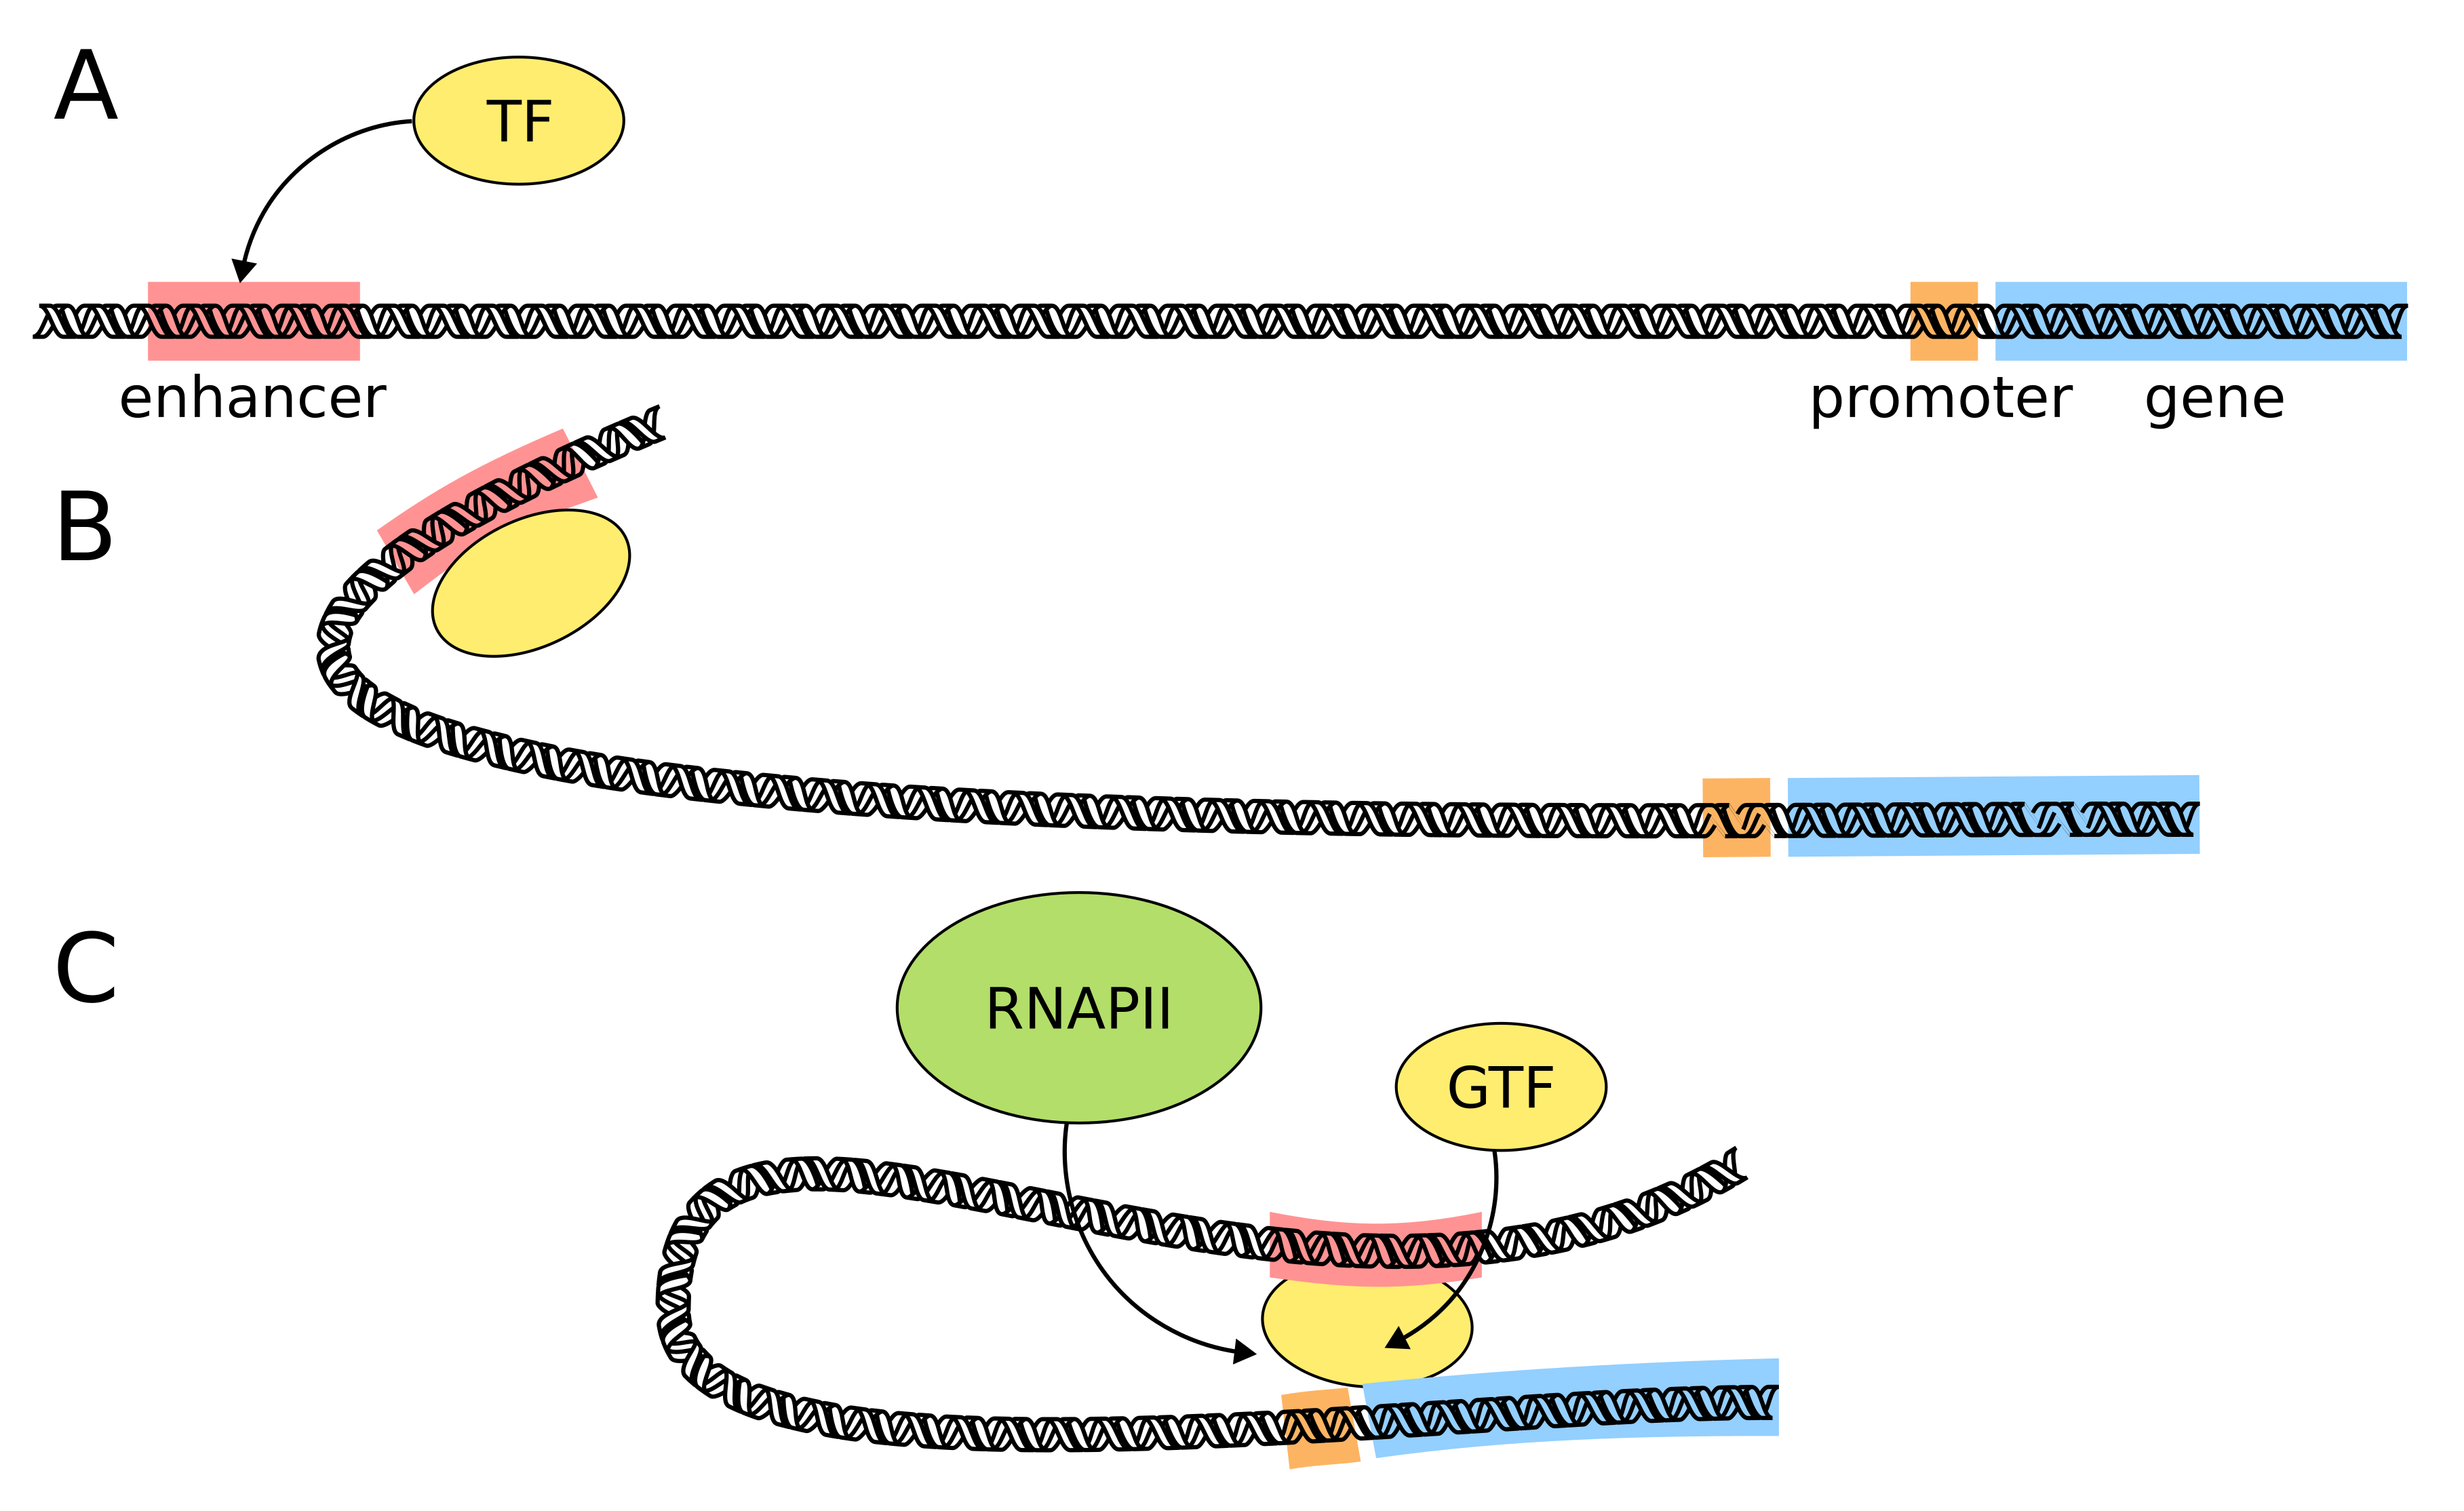
\includegraphics[width=0.8\linewidth]{ch.introduction/imgs/transcription_factor.png}
    \caption{\textbf{Gene regulation by transcription factors.} \textbf{(A)} A gene (blue area) with a promoter upstream (orange) and a "distal" enhancer (red). A transcription factor (TF) binds to the enhancer. \textbf{(B)} The TF causes the DNA to "loop", bringing the enhancer and TF closer to the promoter. \textbf{(C)} Because of the DNA loop, the distal enhancer and promoter are in close proximity, and the TF can increase transcription by recruiting general transcription factors (GTFs) or RNA polymerase II (RNAPII). Usually, multiple enhancers and multiple transcription factors per enhancer are involved, and their combined action regulates gene expression.}
    \label{fig:TF}
\end{figure}

Gene expression is regulated through the combined action of many (cis-)regulatory elements, such as the promoter and enhancers, but also silencers and insulators\cite{Spitz2012}. Silencers have a similar but opposite function to enhancers, they downregulate transcription. Insulators regulate the distances between enhancers/silencers and the promoter. Insulators function by recruiting proteins that create a physical 
barrier, effectively blocking interactions between regulatory elements located on opposite sides of the insulator. An insulator in between an enhancer and promoter can, for instance, block the TFs bound on the enhancer from recruiting GTFs to the promoter.

There are usually multiple transcription factors binding at a single enhancer, and the function of an enhancer should be considered at the combinatorial level. The positioning of motifs in an enhancer is known as the motif grammar, and includes, for instance, the presence (or absence) of certain motifs, the order of these motifs, their orientation, and spacing. Studying motif grammar is a hard problem, as there are many permutations of motifs possible in a single enhancer. Moreover, motif grammar changes based on the cell type, and it is costly to experimentally validate predictions.

\subsection{Chromatin context}

To be able to fit two meters of DNA into each cell, DNA needs to be carefully folded. Chromatin is the term for the structure of DNA, which consists of DNA and proteins. The main proteins in chromatin are histones. Histones are protein complexes around which DNA tightly wraps, forming a structure called a nucleosome. Nucleosomes are the basic units of chromatin (fig. \ref{fig:histones}). Next to the structural role of chromatin,  it also plays an important part in gene expression regulation, and can both promote and inhibit gene expression.

\begin{figure}
    \center
    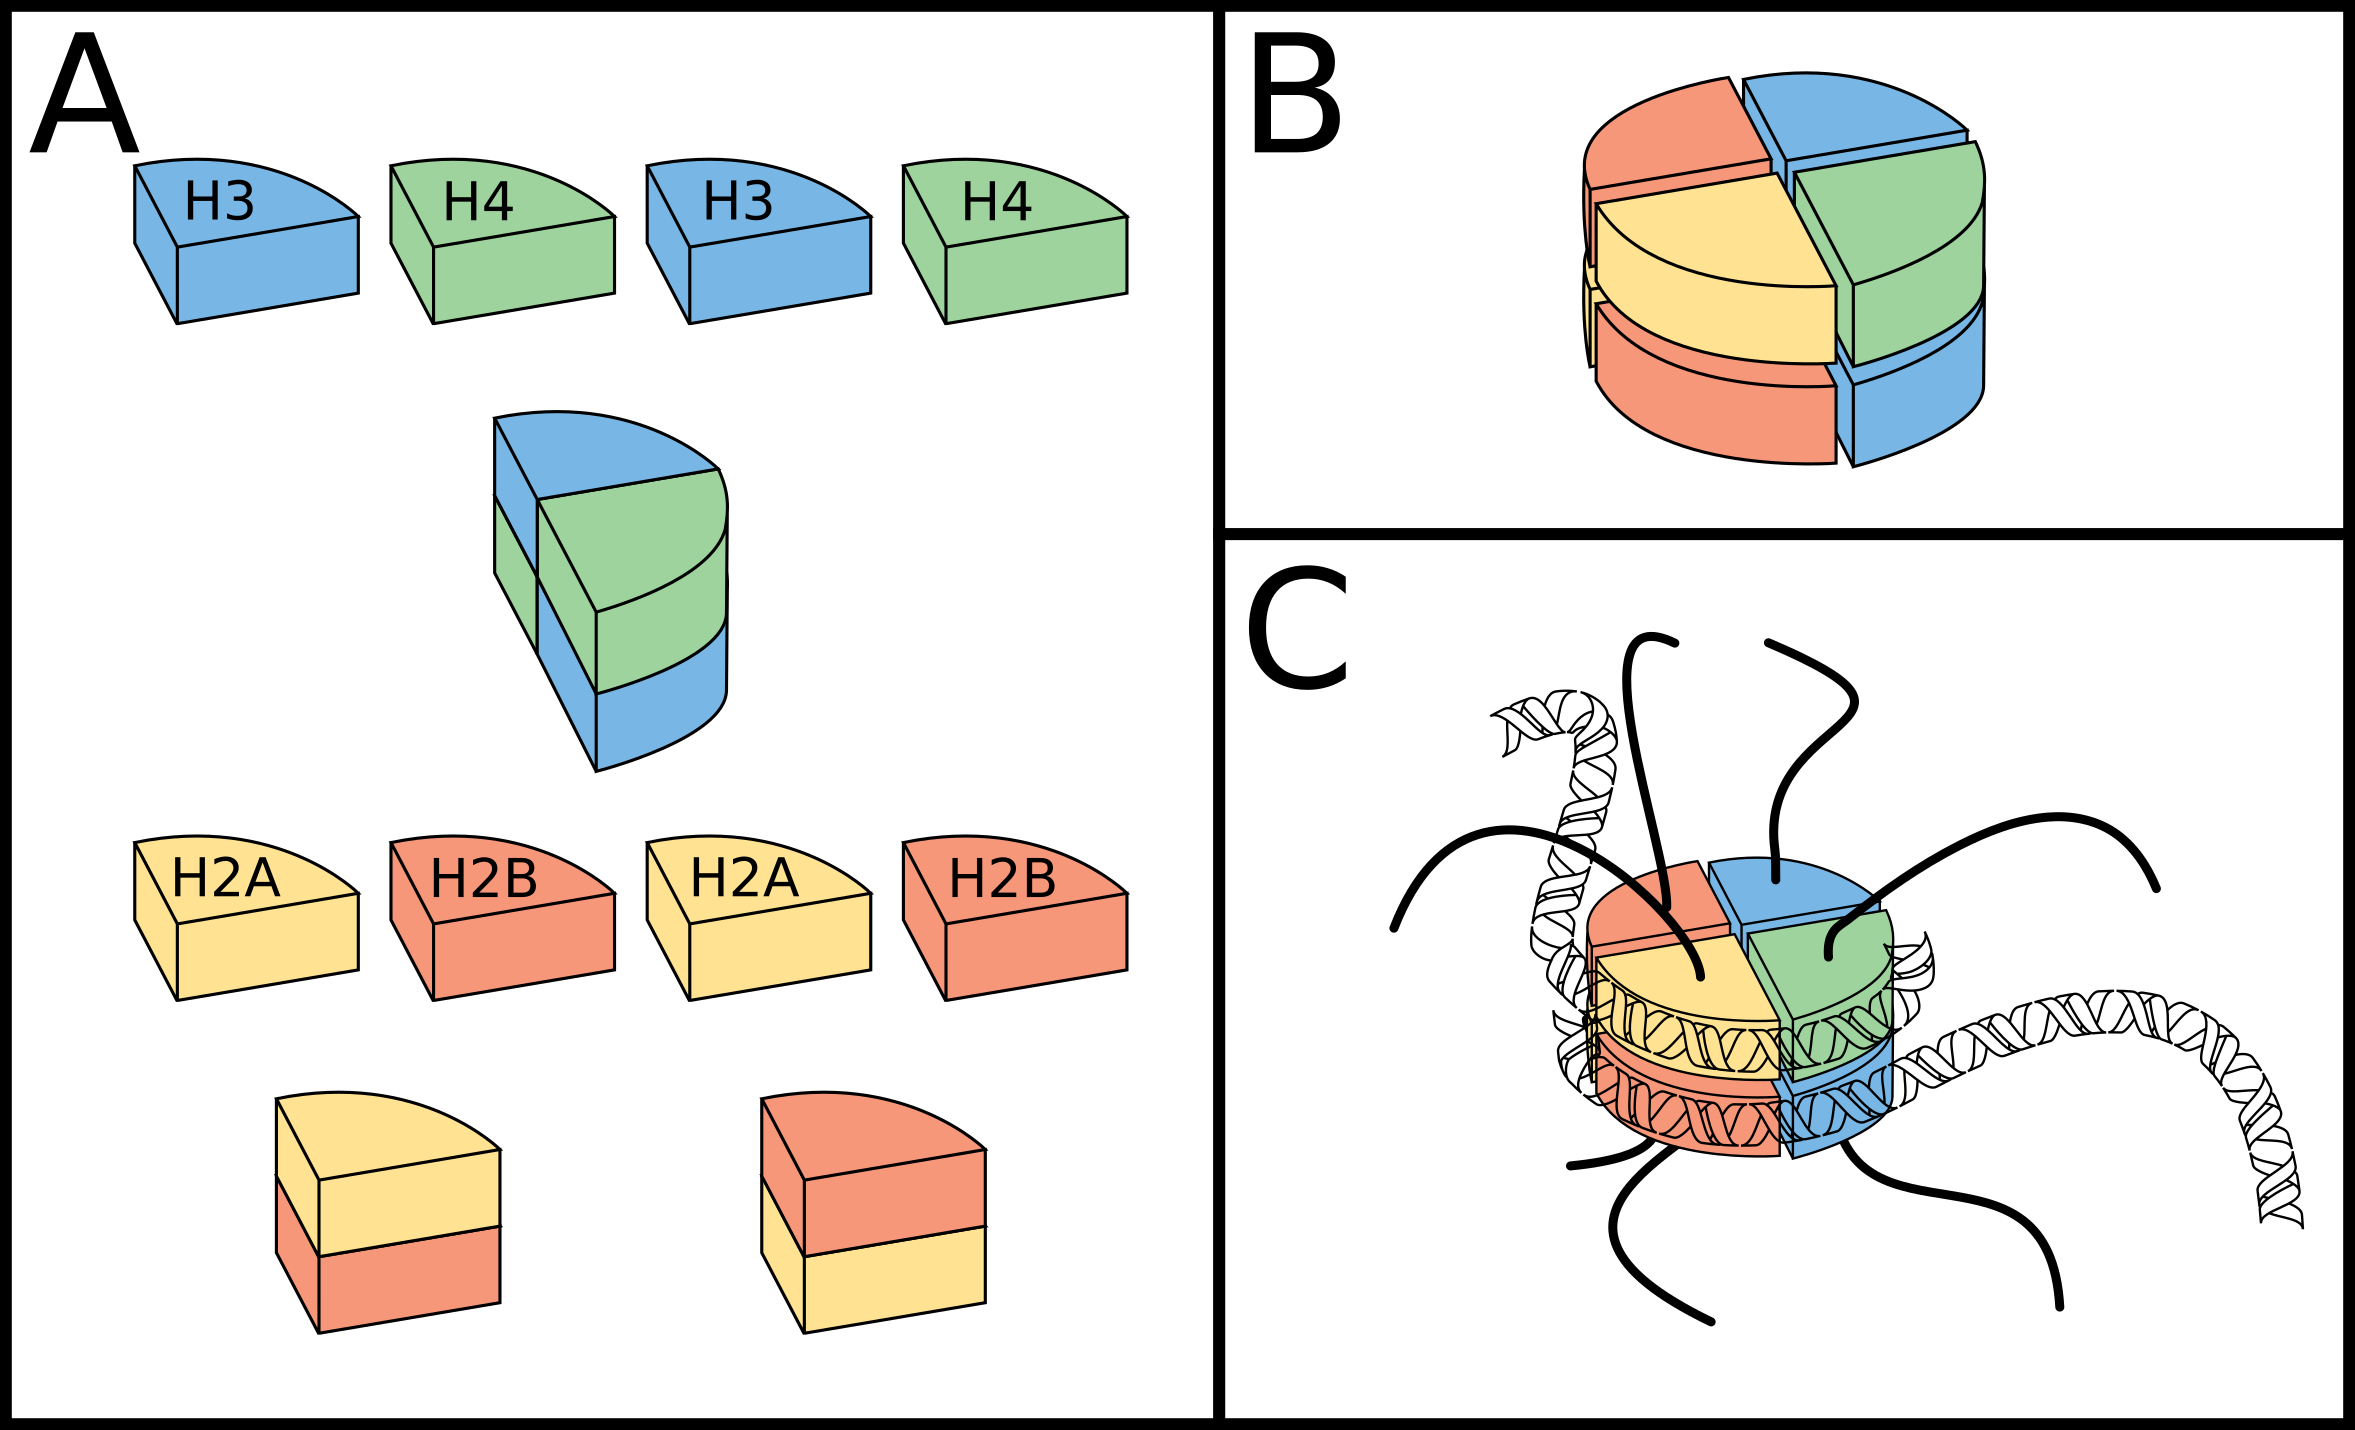
\includegraphics[width=0.8\linewidth]{ch.introduction/imgs/histones.png}
    \caption{\textbf{The nucleosome consists of a histone complex with DNA wrapped around it.} \textbf{(A)} The eight subunits of a histone complex. \textbf{(B)} An assembled histone complex. \textbf{(C)} A histone with DNA wrapped around it. DNA wraps twice around a histone in 146 base pairs. Chemically modifiable tails stick out of the histones, which are important markers and regulators of chromatin state.}
    \label{fig:histones}
\end{figure}

Histones have long protruding tails, that serve as a binding scaffold for protein complexes. These complexes in turn remodel the chromatin, for instance, to condense it, which blocks access of TFs to the DNA. The tails are chemically modifiable, such as by acetylation-, methylation-, and phosphorylation. The way to describe the modifications is by adding the histone number, amino acid, and type of modification. A well-studied modification is H3K27ac, which is the acetylation (ac) of the 27th amino acid, which is Lysine (K), of histone 3 (H3). H3K27ac tends to be associated with an open chromatin structure, allowing easier access to the DNA, and thus promoting the expression of nearby genes\cite{Creyghton2010}. Another example is the H3K9me3 modification, which is the tri-methylation (me3) of the 9th amino acid, Lysine (K), of histone 3 (H3). H3K9me3 is associated with a high nucleosome density and is generally a mark for repressed DNA\cite{Barski2007}.

Nucleosomes are not evenly spread out along the DNA. There are stretches with barely any nucleosomes, called nucleosome-free regions or open chromatin, or regions with a high density of nucleosomes, called closed chromatin or heterochromatin. The general idea is that closed chromatin is so tightly folded that it is difficult for proteins such as TFs to read and bind to the DNA. The other extreme is open chromatin, where (almost) no nucleosomes are present. Here there is nothing to block proteins from accessing the DNA, and open chromatin is generally associated with active DNA\cite{Klemm2019}. In between open and closed chromatin is permissive chromatin, where nucleosomes are present, but the DNA is not folded so tightly that it has become inaccessible. 

Another way chromatin context regulates gene expression is by the specific positioning of nucleosomes. A sequence of 146 base pairs wraps twice around a histone complex. By wrapping around a histone, two motifs at +/- 73 bp distance can suddenly become adjacent. It is thus not surprising that nucleosome positioning is far from random, and plays an important role in gene expression regulation\cite{Jiang2009}.

Finally, another important aspect of gene regulation is DNA methylation, where methyl groups are added to certain regions of DNA. DNA methylation can cause genes to be "silenced" or turned off, as it prevents the cellular machinery from binding to the DNA and initiating gene transcription.

\begin{figure}
    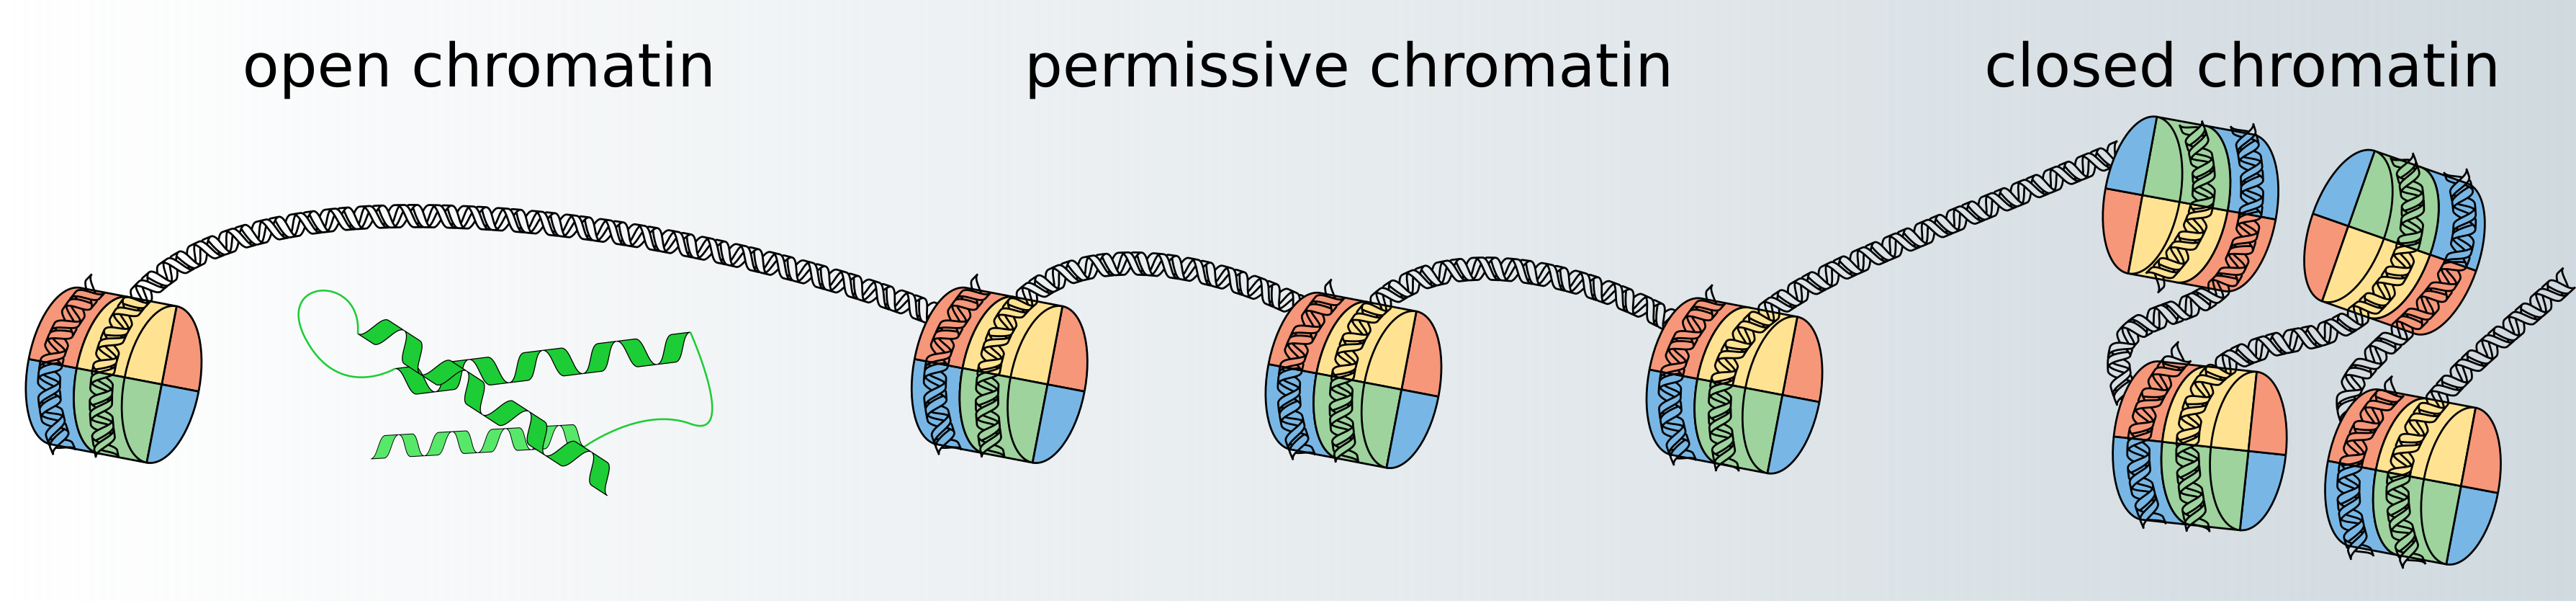
\includegraphics[width=\linewidth]{ch.introduction/imgs/accessibility_horizontal.png}
    \caption{\textbf{Schematic representation of how chromatin context regulates DNA accessibility}. There can be no histones bound, which results in open chromatin. Transcription factors can easily scan the DNA for motifs and bind. Closed chromatin on the other hand is so tightly bound by histones that the DNA has become inaccessible for transcription factors. In between lies permissive chromatin, which, depending on the histone modifications is accessible for transcription factors.}
    \label{fig:accessibility}
\end{figure}

\subsection{Other gene regulatory modes}

There are many other ways gene expression is regulated, such as by regulating RNA degradation, post-translational modifications, and signal transduction. After transcription, RNA exists in the cell and gets translated into protein by ribosomes. Mammalian RNA has a lifetime of several minutes to days\cite{Yu2001}. But to be able to react to environmental changes, a cell is able to mark RNAs for degradation, for instance by poly-A tail removal. 

In addition, the activity and localization of proteins can be regulated by post-translational modifications. These modifications play an important role in fine-tuning the functionality of proteins and their interactions with other molecules. Many different post-translational modifications exist, such as phosphorylation, acetylation, sumoylation, and methylation. These modifications usually influence the protein's stability, shape, activity, and localization. Phosphorylation, for instance, can serve as a switch to activate or deactivate specific protein functions, ubiquitination marks proteins for degradation, and sumoylation is involved in proteins' stability and localization\cite{Mazur2012}.

Finally, chemical and physical signals also play an important role in regulating gene expression. Our bodies react to light by keeping a day-night schedule, produce melanin after exposure to UV light, and grow our muscles after training. A particularly interesting example of how such signals regulate gene expression is the electrical signal that flatworms use during regeneration. A flatworm is a highly regenerative animal, you can cut off its head and tail, and the worm will regrow back its head and tail. It turns out that flatworms make use of an electrical gradient along their body that helps cells decide where in the body axis they are. When one cuts off the head and tail of a flatworm, whilst simultaneously interfering with this electrical gradient, you get flatworms that grow back two heads or tails\cite{Levin2014}.

\subsection{Gene regulatory networks}

Mapping how protein products of genes (e.g. transcription factors) influence the protein level of other genes is crucial for understanding how cellular processes are regulated. A common abstraction to understand gene-gene interactions is a gene regulatory network.

The first concept of gene regulatory networks was proposed by Roy Britten and Eric Davidson in 1969\cite{Britten_1969}. They observed that a cell (i) responds to an external signal; (ii) then produces its own signal as a response; (iii) transmits its own signal to receptors that do not perceive the external signal; (iv) then responds to its own signal, and finally (v) produces a protein as a response. Without modern knowledge of gene regulation, they then predicted what the minimum requirements are for such a system. One of the things they correctly predicted was the existence of transcription factors and promoter sequences. It took Eric Davidson more than 30 years to experimentally validate his original predictions\cite{Davidson_2002}.

Gene regulatory networks come in many forms and shapes but are often modeled and visualized with direct gene-gene interactions (fig. \ref{fig:network}A). This means for instance that the protein product of gene $\alpha$ directly regulates the protein product of gene $\beta$, ignoring all steps, such as transcription and DNA binding, in between. Even though this is a gross oversimplification of gene-gene interactions, these simple models can already exhibit complex behavior. One of the older and more well-known examples of complex behavior from a simple model is a Turing pattern, first described by the famous computer scientist Alan Turing\cite{Turing1952}. One specific Turing model, the Gierer-Meinhardt model, consists of two genes, gene $\alpha$, and gene $\beta$, where gene $\alpha$ upregulates itself and gene $\beta$, but gene $\beta$ inhibits gene $\alpha$ (fig. \ref{fig:network}B). When modeling this simple two-gene network in a spatial setting it produces complex patterns (fig. \ref{fig:network}C), of which similar patterns have been observed in nature, such as the skin pattern of a pufferfish (fig. \ref{fig:network}D).

\begin{figure}[H]
    \center
    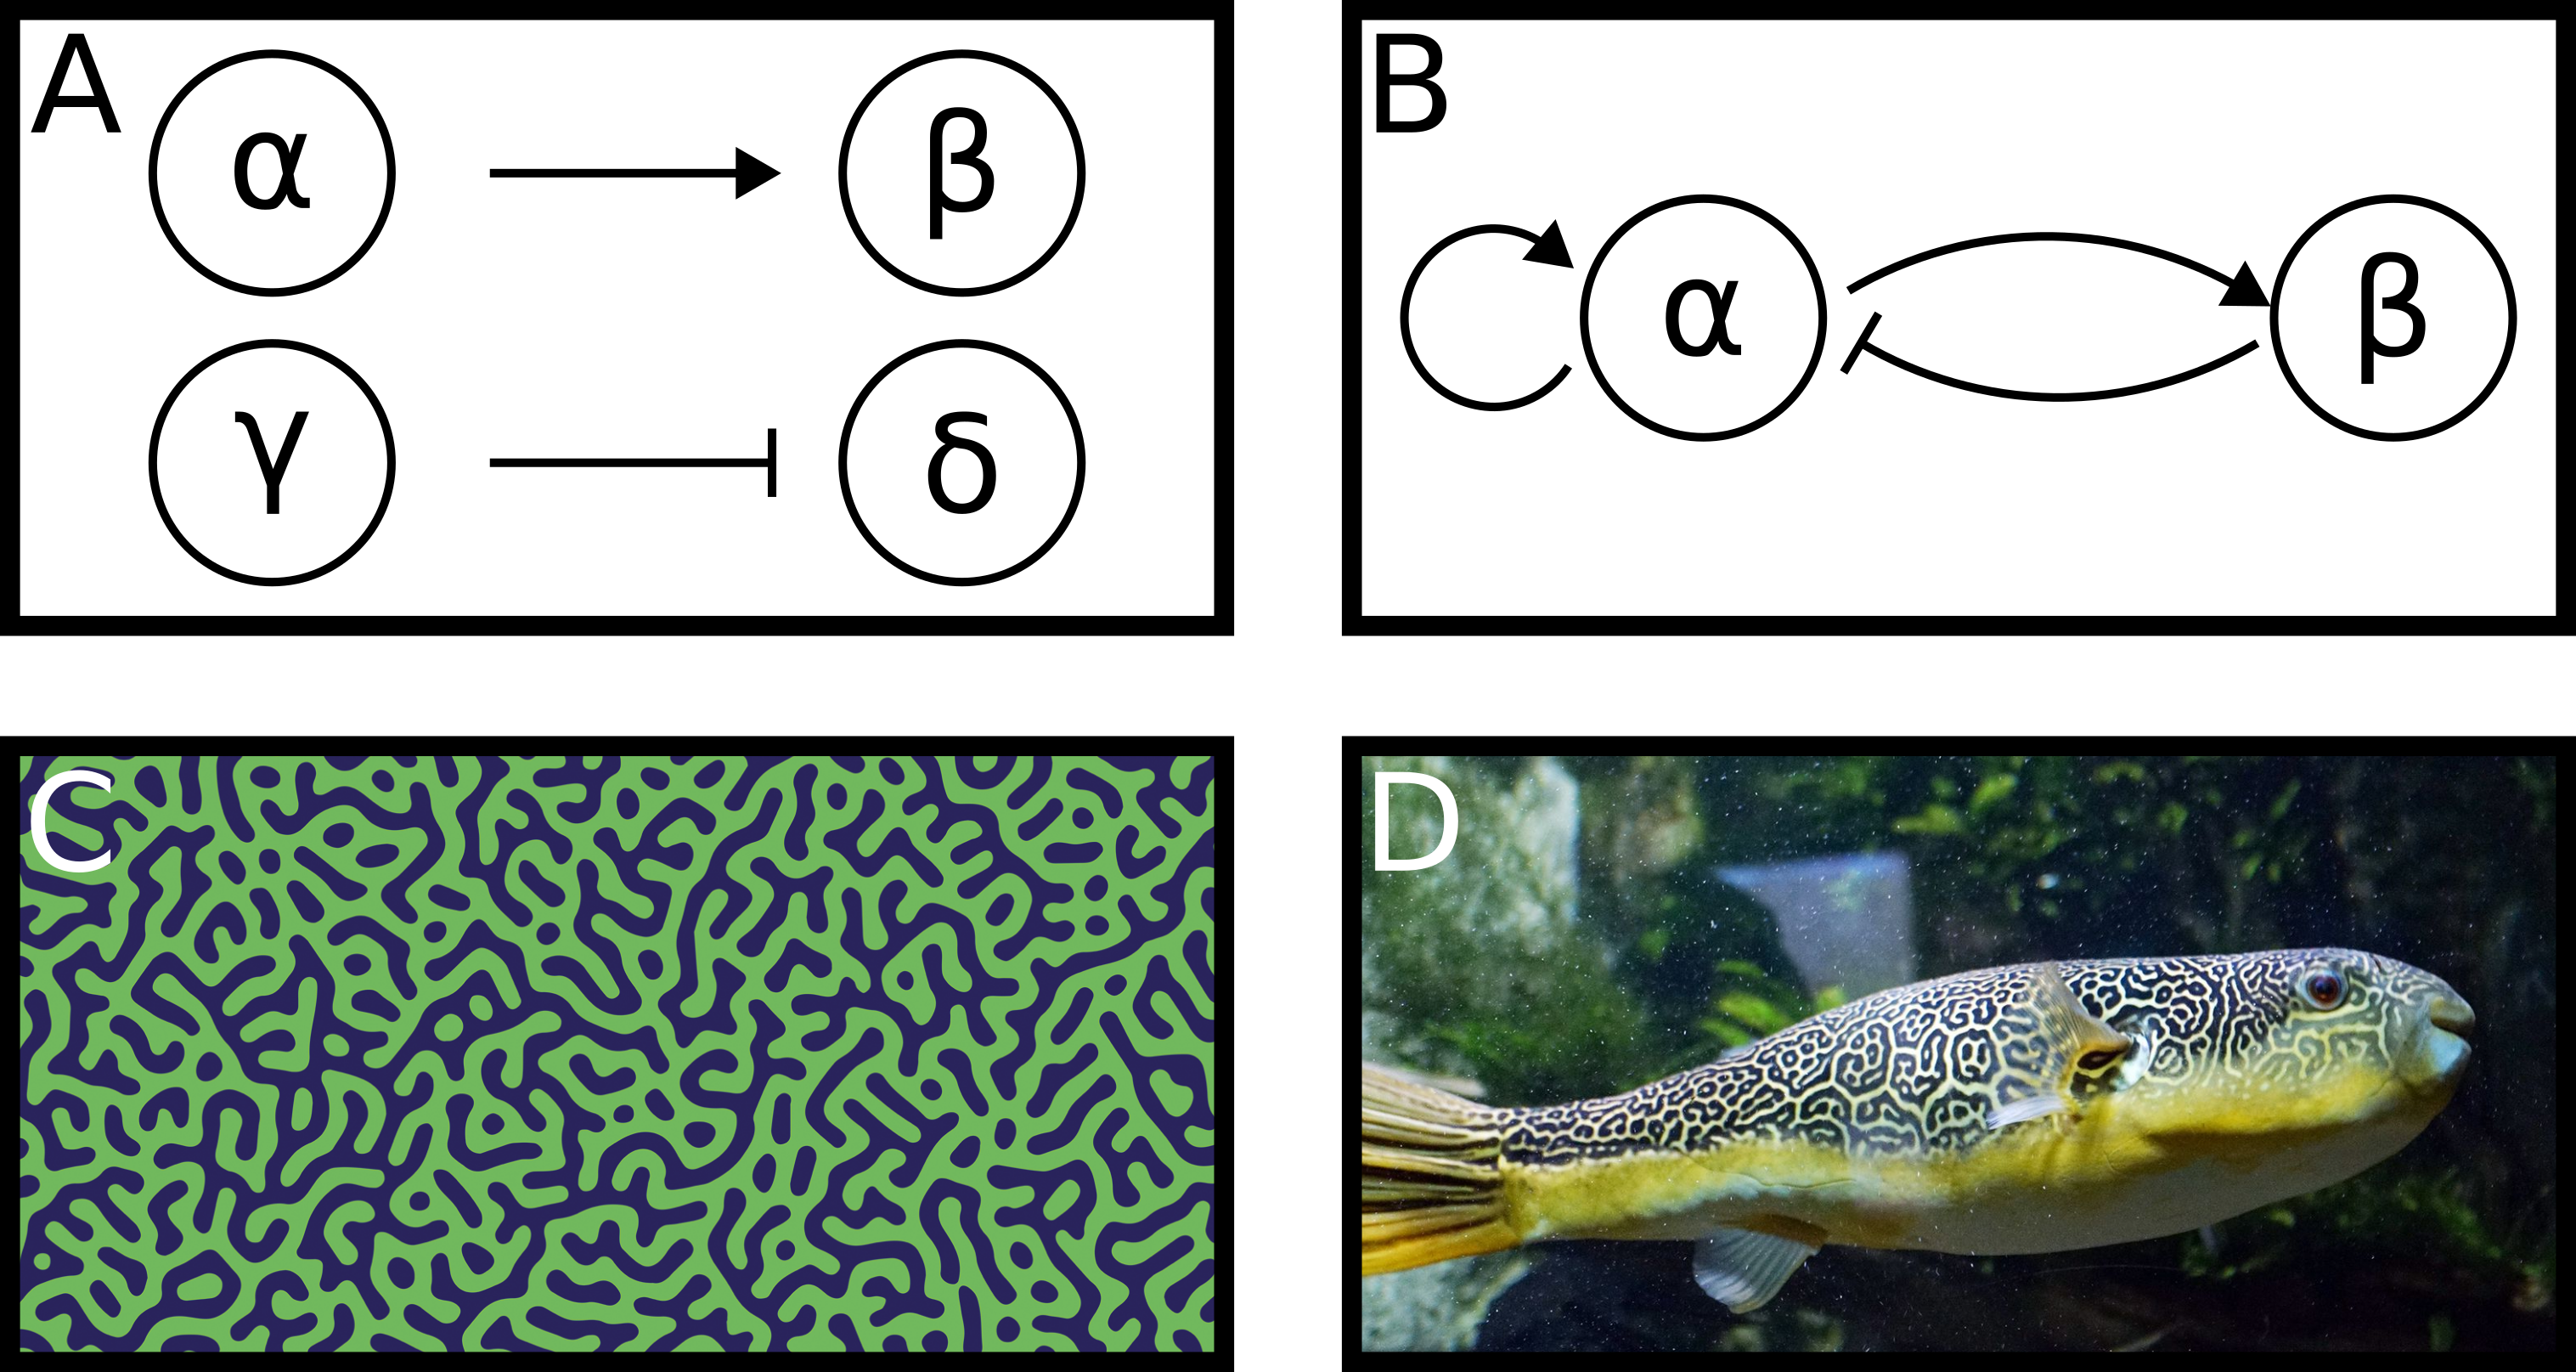
\includegraphics[width=0.8\linewidth]{ch.introduction/imgs/network.png}
    \caption{\textbf{Basic gene regulatory networks.} (\textbf{A}) the standard schematic way of representing gene-gene interactions. Gene $\alpha$ upregulates gene $\beta$, and gene $\gamma$ downregulates gene $\delta$. (\textbf{B}) Gierer-Meinhardt gene regulatory network, where gene $\alpha$ upregulates itself and gene $\beta$, and gene $\beta$ downregulates gene $\alpha$. (\textbf{C}) Simulation of the Gierer-Meinhardt gene regulatory network in a spatial context. (\textbf{D}) A Mbuna pufferfish with Turing pattern. Turing pattern from: https://www.nature.com/articles/s43588-022-00306-0 and pufferfish photo taken by Tiia Monto: https://en.wikipedia.org/wiki/Mbu\_pufferfish\#/media/File:Tetraodon\_mbu\_2.jpg}
    \label{fig:network}
\end{figure}

Mapping the relations between genes is a hard problem and unfeasible to do by hand. Not only can potentially any gene have an (in)direct effect on any other gene, but the potential interactions also depend on the cell type. The 20.000 human protein-coding genes have 20.000$^2$=400.000.000 potential direct interactions, and if we consider indirect interactions, cell type-specific interactions, and combinatorial interactions the number of potential gene networks explodes. To infer gene interactions at scale and make sense of the resulting networks we \textit{have} to make use of computational tools. The most common approach so far has been to measure RNA expression in a combination of settings and correlate the RNA expression of genes over these settings \cite{Zhang_2005,Margolin_2006}. Correlations above a certain threshold would indicate an (in)direct gene regulation. Adding more information to these networks, such as the chromatin state around genes\cite{Xu_2020,Kamal_2021}, improves the resulting networks. However, practically all gene regulatory network inference approaches compare cell states (e.g. liver vs. skin), so the inferred gene networks are specific for these comparisons. In chapter 2 we discuss the latest developments in gene regulatory network inference.

\section{Genomics analysis}

A genomics project can be broken down into two main stages: wet lab work,  and computational analysis. The wet lab phase involves hands-on experimentation with physical materials like chemicals and biological samples, DNA isolation, and DNA sequencing. In contrast, the dry lab phase is concerned with the computational interpretation and analysis of the data generated by the wet lab.  In this thesis, three different types of sequencing assays have been used and analyzed (ATAC-seq, ChIP-seq, and RNA-seq), and here I will briefly explain their wet lab and computational analysis aspects. 

\subsection{Wet lab}

Assay for Transposase-Accessible Chromatin using sequencing (ATAC-seq) is a method to measure genome-wide accessibility\cite{Buenrostro_2015}. Accessible DNA is generally associated with active DNA, and vice versa. ATAC-seq works by adding a protein called Tn5 transposase to a sample. This protein then proceeds to randomly cut up the genome. However, if a piece of DNA is inaccessible, for example, because a histone modification is blocking access, the Tn5 can not reach the DNA to cut it. Small DNA sequences thus represent accessible DNA as they could be cut. After treating DNA with Tn5, one then isolates the small DNA fragments (+/- 1.000 base pairs long), which are then ready to be sequenced.

Chromatin ImmunoPrecipitation sequencing (ChIP) is an assay to measure proteins in proximity to DNA\cite{Robertson_2007}. These proteins are usually transcription factors or histone modifications. It works by first fixating (gluing together) the chromatin with formaldehyde. Afterward, you break the DNA into small pieces of +/- 200 bp long. You then add proteins that bind to your protein of interest (antibodies) and filter out all the DNA sequences with bound antibodies. By using, for instance, magnetic antibodies one can filter out the antibodies with magnets. As the final step, the DNA, proteins, and antibodies need to be separated, and the remaining DNA fragments can be sent for sequencing.

RNA-seq is a method to estimate which gene transcripts are present in a sample and in what quantity\cite{Nagalakshmi2008}. The amount of RNA transcripts of a gene can be used as a proxy for both the level of gene regulation as well as for the number of protein product that is present in a sample. RNA-seq works by first filtering out all the RNA in a sample, and then converting the RNA into DNA by reverse transcription (see fig. \ref{fig:central_dogma}. The resulting DNA then represents the number of gene transcripts for a gene, and can then be sequenced.

\subsubsection{Sequencing}

Sequencing refers to laboratory techniques that determine the order of nucleotides in a DNA sequence. Here we will focus on the sequencing by synthesis method, although various other techniques, such as Sanger, Oxford Nanopore, and PacBio, also exist. Sequencing happens on a surface known as a flow cell, and to bind the DNA sequences to this surface, the process starts with the addition of adapters to both ends of each DNA strand. Subsequently, the DNA is thinly spread across the flow cell, and the adapters function as anchors, fixing the DNA to the flow cell. The DNA strands then get amplified by PCR, and as the adapters are also amplified, the resulting sequences are anchored in close proximity to the original. This leads to clusters of identical DNA sequences forming concentrated spots on the flow cell. The flow cell is then subjected to heat, causing the DNA strands to become single-stranded. One at a time, fluorescently labeled nucleotides are added to the flow cell, which, in chronological order, makes the DNA double-stranded again. Each of the four nucleotides has its own specific color which gets emitted when it is incorporated into the DNA. Throughout this process, a camera captures the emitted colors from each spot. The final output of sequencing is a video, where the order of colors emitted from each spot corresponds to the sequence of DNA.

\subsection{Dry lab}

The resulting video is then converted to a file with as many lines as there were spots on the flow cell, where each line represents a DNA sequence (fastq). First, one needs to remove the sequencing adapters of these sequences, to then map where the reads fit onto the genome. Mapping to the genome is a compute-heavy task, as fastq files generally contain several millions of reads, and genomes are large (billions of nucleotides). After mapping, one ends up with a file that aligns each read to a position in the genome. Generally, the next step is to assign features to the genome based on where many reads map. For RNA-seq this is usually easy, as we already know where the genes are, and we can simply count the number of reads aligned inside each gene for each sample. For ATAC-seq and ChIP-seq experiments we generally do not know the regions of interest yet. So we first need to select the regions of the DNA of interest. This is usually done by so-called peak-calling algorithms \cite{Zhang2008,Stovner2019_epic,Tarbell2019}. These algorithms look for regions (peaks) where the number of reads mapped passes a statistical threshold. The results of different samples in ATAC, ChIP, and RNA-seq experiments are usually aggregated in a table, where each row represents a gene/peak and each column a sample. The number in each cell then represents the number of reads mapped for that gene/peak and sample combination.

After obtaining a table with values for each sample, it depends on the research question what further steps are needed. If one for instance is interested in liver development and has generated a liver time-series it is common to infer the liver gene regulatory network. If one, on the other hand, is interested in the difference between two relatively similar conditions, for instance, healthy vs. sick livers, it is common to do a differential expression analysis on the table. Gene regulatory network inference based on RNA-seq usually happens by correlating gene expression over time. Gene-gene correlations that pass a certain threshold are assumed to be causal. Gene regulatory network inference on ATAC-seq or histone ChIP-seq is usually done by doing a TF-motif analysis on the peaks. Ideally, one combines both RNA-seq and ATAC/CHIP-seq for more accurate gene networks. Differential expression analysis on the other hand provides a list of all the differentially expressed genes/peaks. These features are then indicators of the possible differences between samples and are targets for further investigation and treatment.

\begin{figure}
    \center
    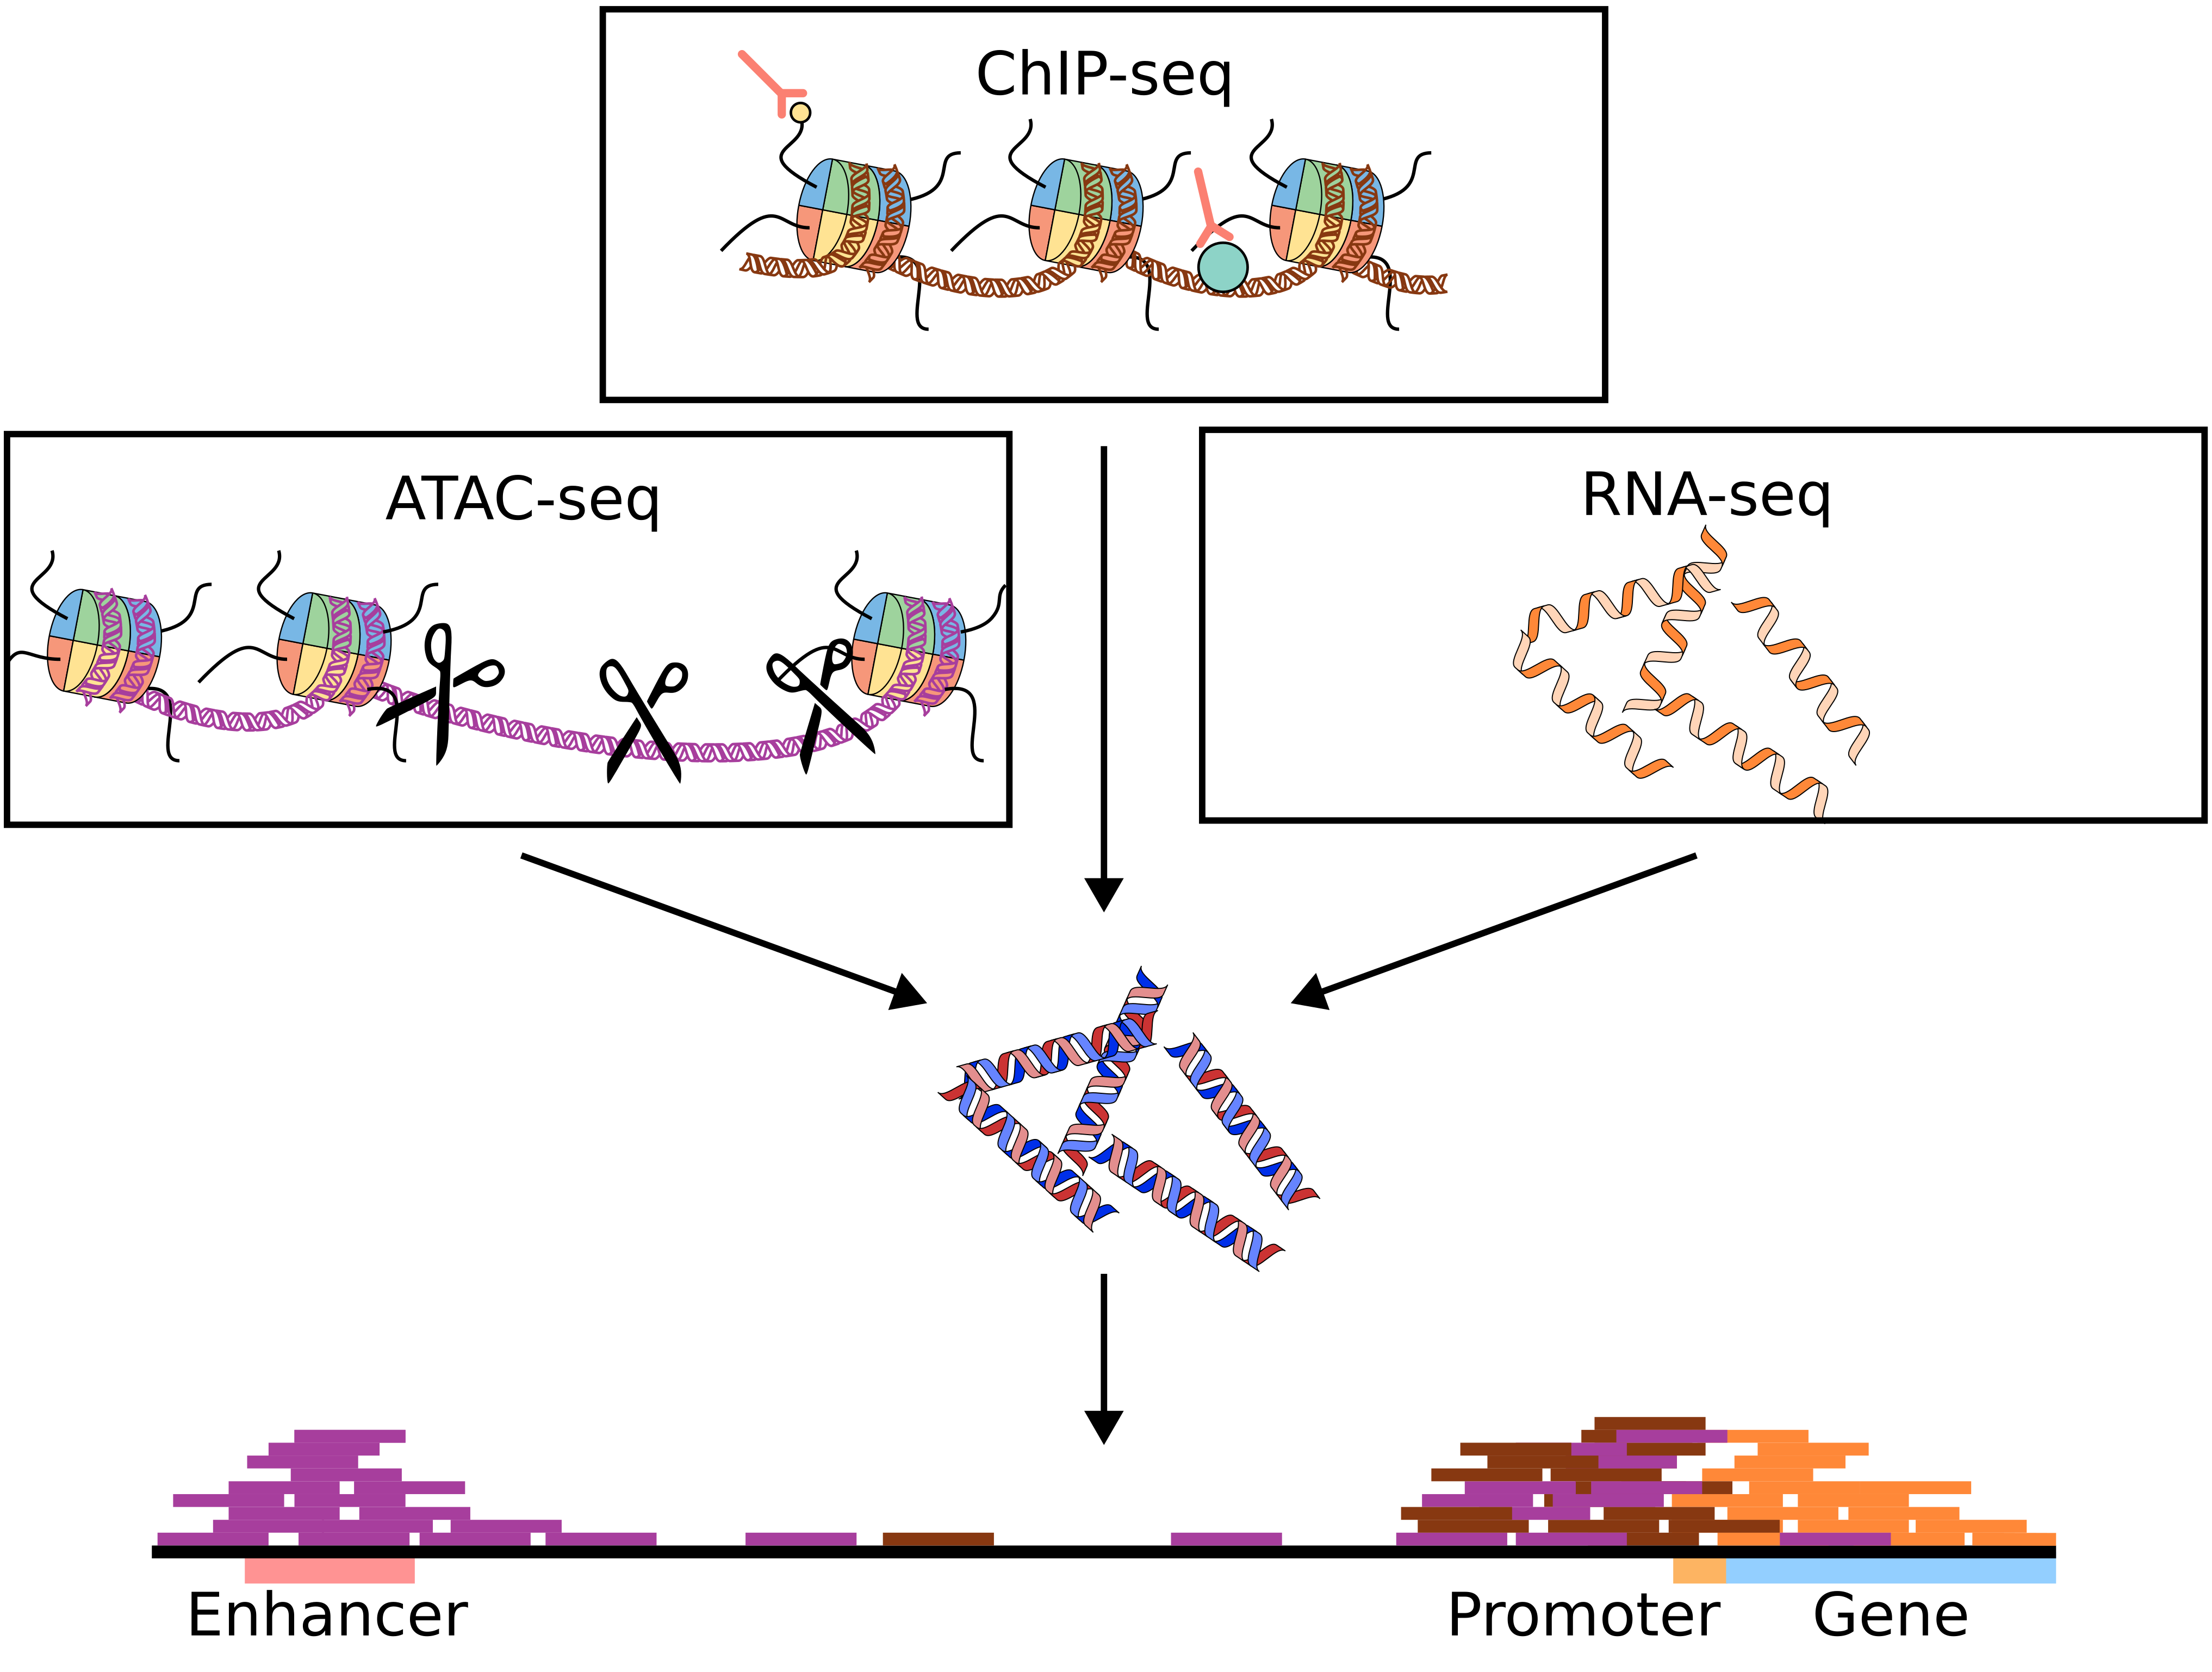
\includegraphics[width=0.8\linewidth]{ch.introduction/imgs/analysis.png}
    \caption{\textbf{Schematic overview of ATAC-seq, ChIP-seq, and RNA-seq and their computational analysis.} ATAC-seq is a technique that cuts out accessible DNA. ChIP-seq is a way to isolate DNA sequences with specific proteins bound. RNA-seq is a technique for the estimation for the number of transcripts per gene. In the wet lab, all three methods produce DNA sequences that need to be sequenced. After sequencing the DNA gets computationally mapped to the genome by the dry lab, after which the real analysis starts. }
    \label{fig:analysis}
\end{figure}

In Chapter 3 and Chapter 4, I introduce dry lab tools seq2science and qnorm respectively. Seq2science is a preprocessing pipeline, that only requires fastq files as input, and runs an extensive analysis on them. Qnorm is a quantile normalization package, a common normalization technique to apply on count tables. Seq2science and qnorm streamline a significant portion of the dry lab workflow, resulting in standardized analyses and freeing up additional time for data exploration.

\subsection{Single cell}

A major downside of traditional sequencing is that it requires a lot of input DNA to be sensitive. For this reason, usually larger samples/biopsies of tissues are sequenced. The problem with this is that the measured signal is a compound signal of all the cells present in a sample. If we were to take a biopsy of the liver, it would consist of a combination of liver cells (hepatocytes), blood cells, fat cells, etc. This is why this type of sequencing has become known as bulk sequencing. Relatively recently, new techniques have been developed to separate all cells in a sample and perform RNA- or ATAC-seq on each cell separately\cite{Buenrostro2015_sc,Tang2009}. This type of data gives unprecedented precision in analyses and has been welcomed as a major improvement over bulk sequencing.

A major downside of single-cell sequencing, however, is that the data analysis is significantly harder. Whereas originally one would compare for instance a healthy liver vs. a sick liver, now there are thousands of liver cells separated over multiple cell types to compare. Moreover, the hardware that was used for the original bulk analyses is suddenly not powerful enough to deal with the enormous increase in data. Furthermore, statistical methods developed for bulk analyses are not appropriate anymore, as for instance, a cell has two copies of each chromosome, so genomic assumptions of continuous distributions of reads are broken. Moreover, single-cell sequencing has the problem that it is extremely sensitive to batch effects, with major differences between who, how, and when the cells were sequenced.

Regardless of these downsides, single-cell sequencing is a promising technique that has been quickly adopted in the field of genomics. It has given the field a new appreciation for the complexity of biology. In chapter 7 we TODO SCEPIA

\section{Evolutionary development (evo-devo)}

A single fertilized egg cell multiplies and develops into a complex collection of trillions of cells by the time we reach adulthood. How does each cell know where it is positioned in the body and what to develop into? The field of evolutionary development (evo-devo) studies development from an evolutionary point of view. In the 1980s scientists discovered a set of genes in fruit flies, which when mutated, were responsible for strange bodily transformations. A mutation in these genes caused flies to grow legs instead of antennae from their mouths\cite{Schneuwly1987} or flies to develop a second pair of wings\cite{Weatherbee1998}. This work was revolutionary at the time as it showed that (precursor) antennae cells contain all the information necessary to build legs. The group of genes responsible for these mutations are transcription factors known as hox genes.

The embryonic development of a fruit fly starts as a worm-like larva consisting of multiple repeated segments. The gene expression of hox genes determines the identity of each  and guides its growth. For example, the \textit{lab} hox gene is expressed at the frontal part of the larva, indicating surrounding cells this area will develop into the mouth of the fly\cite{Hughes2002}. Similarly, the \textit{Antp} hox gene indicates leg formation and is expressed in the mid-section of the larva. Interestingly, hox genes are found in nearly all animals, where they play an important role in the spatial organization of the organism. What makes Hox genes particularly fascinating is that their order on the chromosome is the same as the spatial ordering along embryos. This concept is called spatial colinearity, something we have no clear understanding of\cite{Gaunt2015}.

\begin{figure}
    \center
    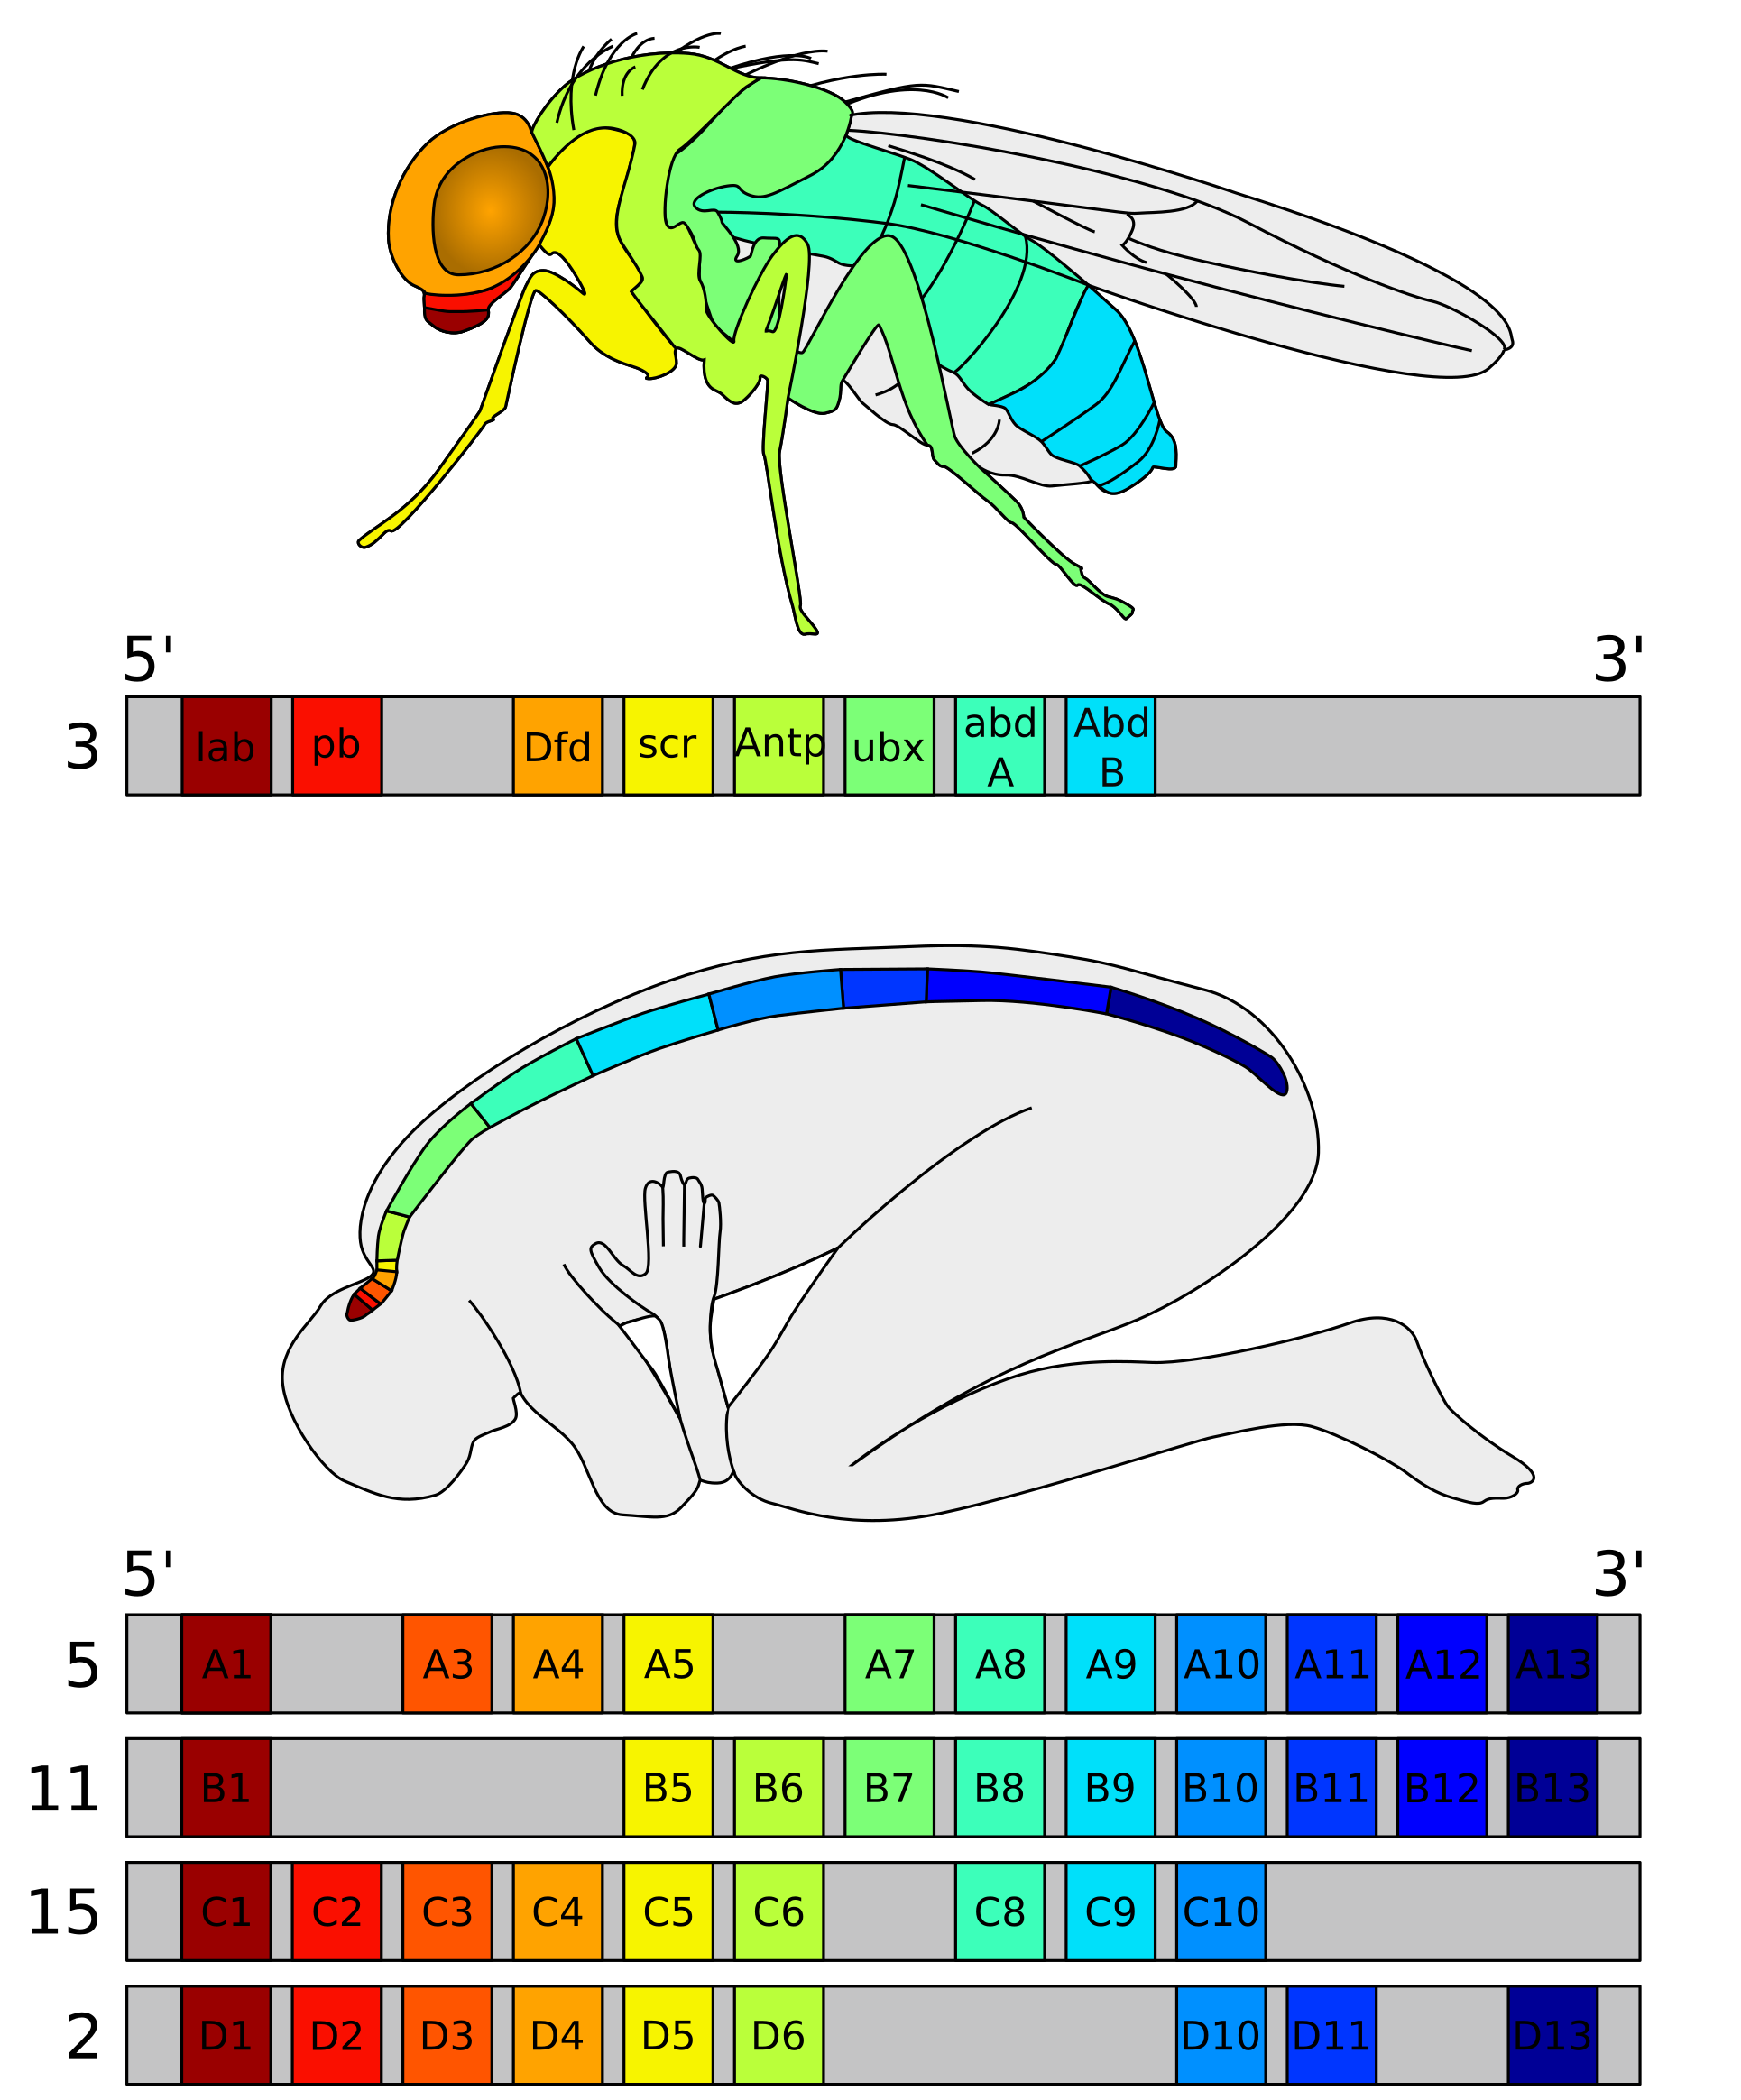
\includegraphics[width=\linewidth]{ch.introduction/imgs/hox.png}
    \caption{The genomic ordering of hox genes in fruit fly and human, and their colinearity in expression. All the hox genes for the fruit fly lay on chromosome 3. The human genome has had two genome duplications since the last common ancestor with fruit flies, so the hox genes are spread over four chromosomes (5, 11, 15, and 2). Even though some hox genes got lost on some chromosomes, their ordering has remained the same.}
    \label{fig:hox}
\end{figure}

Another remarkable family of transcription factors is the pax transcription factors. While the hox transcription factors are generally responsible for the anterior-posterior (head-to-tail) axis, the pax transcription factors are involved in the development of structures like the eyes, ears, nervous system, and other organs. The most-studied of the family is the pax6 transcription factor, which is involved in eye development and is highly conserved for bilateria (e.g. fruit flies, frogs, and humans). Injecting pax6 into a developing frog embryo results in an extra eye on the spot of the injection\cite{Chow1999}.

The observation that single mutations can cause such large changes in body plans, in combination with the fact that the responsible genes are deeply conserved among species, shifted the way we think about evolution. Speciation does not have to happen through a combination of many small incremental mutations, but a few mutations, for instance, in the hox or pax genes, can cause major changes. This is now the basis of the scientific field of evo-devo.

\subsection{The hourglass model and the phylotypic stage}

Where the molecular observations of the hox and pax genes are a relatively recent addition to the field of evo-devo, the oldest observations in the field are based on the morphology (shape) of embryos. Ernst Haeckel has done the most famous and influential observations in the field of evo-devo in the 1800s\cite{haeckel1866}. Through a series of observations and drawings of the embryonic development of different vertebrates, Haeckel noticed a stage early in development where all vertebrates appear morphologically similar. This stage is now known as the phylotypic stage (see figure \ref{fig:haeckel_wide}). The Origin of Species, \textit{the} book by Charles Darwin in which he proposes the evolution theory, was only published a decade before these observations, and the idea of a scala naturæ (the ordering of species into higher and lower species) was still prevalent at that time. Haeckel thought his observations could unify the scala naturæ and the evolution theory, and came with a refinement of the recapitulation theory. Haeckel proposed that embryos of higher species consecutively develop from embryos of lower species into embryos of higher species. For example, a human embryo, which would be the highest and most developed species, would first develop into a fish embryo, then a reptile embryo, and finally into a mammalian embryo. This would explain why, for instance, gills and tails develop in human embryos, to then later disappear. The recapitulation theory unifies the scala naturæ with evolution, as the higher species are more evolved than the lower ones. Haeckel was a strong proponent of eugenics and proposed an ordering in human races, where the Germanic race, coincidentally the race Haeckel belongs to, was listed all the way at the top\cite{Levit2020}. The recapitulation theory was already controversial at the time it was proposed and is refuted by the contemporary scientific community. Nevertheless, the notion of a morphologically conserved stage early in development is prevalent to this day.

\hvFloat[doublePage,capWidth=n,
capPos=bottom,bindCorr=0.0cm]{figure}
{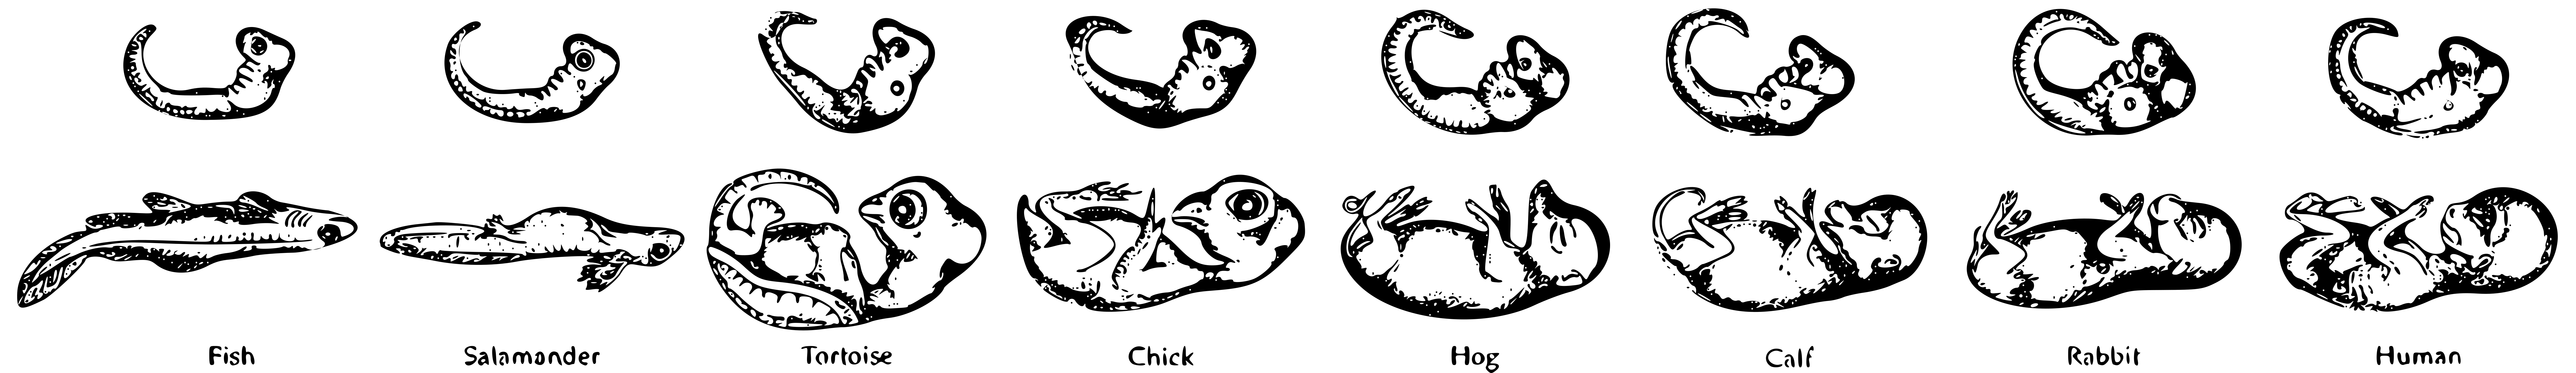
\includegraphics[width=2.2\textwidth]
{ch.introduction/imgs/haeckel_wide.png}}
[accessibility schematic overview]
{Adaptation of George Romanes's 1892 copy of Ernst Haeckel's embryo drawings. The upper row shows early embryos in the phylotypic stage, while the bottom row shows a later stage. Note how all the embryos appear similar in the phylotypic stage. Haeckel has been accused of fraud, amplifying the similarities at the phylotypic stage, with both supporters\cite{Richards2008} and opponents of his drawings\cite{Pennisi1997}}{fig:haeckel_wide}

In the same time period, Karl Ernst von Baer proposed an alternative theory of embryonic development. Von Baer was strongly opposed to Haeckel's recapitulation theory. He noted, for instance, that a yolk sac is present during bird embryonic development, but not for frog embryonic development. This is inconsistent with the recapitulation theory as frogs were considered a higher species than birds. Von Baer's opposing theory consisted of four main rules, or laws\cite{baer1828}. His first law, for instance, states that \textit{the more general characters of a large group appear earlier in the embryo than the more special characters}. This means that as an embryo develops, it first develops its oldest phylum-specific features, to then respectively develop its class, order, family, and species-specific features. Simply put, embryos of related species become increasingly diverse as development proceeds. Von Baer did not believe in the idea of a single common ancestor for all life on earth, as he believed the differences between some species, e.g. humans and sponges, to be too large to be bridged by evolution.

Even though the theories of Von Baer and Haeckel are dismissed by contemporary biologists, their observations of a morphologically conserved stage in development remain intriguing and have led to the formulation of the hourglass model of development. The hourglass model is based on the model proposed by Paul Medawar in 1954\cite{Medawar1954}. Medawar argues that somewhere mid-embryogenesis is the most morphologically conserved stage for vertebrates. This stage corresponds to Haeckel's phylotypic stage, but, different from Haeckel's recapitulation theory, different species are thought to be more diverse both before and after the mid-embryogenesis state. The phylotypic stage coincides with the formation of the basic body plan, so it is a popular hypothesis that hox genes are responsible for this conserved stage. Recently, molecular evidence has been generated that gene expression between different species is most similar at the phylotypic stage \cite{Levin2016,marletaz2018,Mayshar2023,Liu2021,DomazetLoso2010,Irie2011,Kalinka2010,Piasecka2013,Uesaka2019}. This has led to the idea that the phylotypic stage is not just morphologically conserved, but also conserved on the level of gene expression and regulation. In chapter \textbf{TODO 1 and 2} I discuss the current statistical methods that estimate this molecular conservation, and by careful re-analysis, I demonstrate that the used methodology is biased. This in turn means that the conclusions the original authors draw about the phylotypic stage and the molecular hourglass model are unfounded. 

\section{Thesis overview}

This thesis focuses on the computational analysis of (evolutionary-) developmental processes. The current chapter (\textbf{chapter 1}) served as a general introduction to the scientific fields of computational genomics, gene regulation, and evolutionary development.  

In \textbf{chapter 2} I review the current computational approaches to model and understand gene regulatory networks in development. Current computational gene regulatory network inference methods perform poorly, and thus new approaches are needed. I highlight three recent developments for gene regulatory network inference which I expect to improve the power of these methods; multi-omics networks, single-cell data, and artificial neural networks. Multi-omics data partially solves the curse of dimensionality by constraining the problem and providing more data. Bulk sequencing measures the compound signal of multiple cell types. Single-cell sequencing, on the other hand, separates the signal per cell type, so cell-type-specific networks can be made and the data contains a purer signal. Artificial neural networks can model more complex gene-gene interactions than the current approaches. By combining these three approaches I expect future gene regulatory network inference methods to predict better networks.

In \textbf{chapter 3} I discuss the implementation of seq2science, a next-generation pre-processing workflow. Seq2science supports some of the most common assays, such as RNA-seq, ChIP-seq, and ATAC-seq, integrates with public databases, and reports an extensive quality control report. Seq2science has been tested on a wide array of different species and genome assemblies, and I show examples of common analyses that seq2science supports out of the box. Seq2science has an extensive user base\cite{Bright_2021,Xu_2020,Wester2021,SantosBarriopedro2021,Heuts2023,Tholen2023,Harlaar2022,LunaVelez2023,Neikes2023,Vierboom2021,Smits2020,Smits2022,Heuts2022,Rother2023}, is downloaded over 50K times through Bioconda, and has more than 120 ``stars'' on GitHub.

In \textbf{chapter 4} I discuss the implementation of qnorm, a Python quantile normalization package. Quantile normalization is the process of fitting multiple distributions onto their average distribution. Python did not have a quantile normalization package yet, and the implementations on public fora about how to do quantile normalization did not resolve ties properly. Qnorm is fast-ish and scales to infinitely large tables as it can swap memory to disk.

In \textbf{chapter 5} I discuss the molecular basis of the phylotypic stage and its related models. I explain how the current definition and analyses of the phylotypic stage are ambiguous, as they do not distinguish within-species effects from between-species effects. For this reason, I propose that any study of the phylotypic stage includes at least a within-species comparison, a within-phylum comparison, and a between-phyla comparison. By applying these comparisons I find important flaws in the interpretation of previous results. I highlight three examples where the within-species pattern is enough to explain the between-species pattern. Moreover, I find that a supposed between-phyla effect, the mid-developmental transition, is a statistical artifact. Finally, I question the general validity of the current approaches to studying the phylotypic stage, as they are gross oversimplifications of the biological complexity during development.

\textbf{Chapter 6} is a short criticism of a quantitative study of morphological features in relation to the phylotypic stage. The original study finds support for an inverse hourglass model for mammalian embryonic development. However, with simulated data with no particular temporal conservation, I find nearly identical results. The methodology of the original study is biased towards the inverse hourglass, and as such I see no support for their claim of an inverse hourglass model of conservation.

In \textbf{chapter 7} (scepia)

Finally, in \textbf{chapter 8} I summarize and discuss the results described in this thesis, and give future perspectives on the field.
